% A. Rat — rung one. A lab rat who only wants a cure, drawn as the smallest
% thing on the ladder that still has teeth.
%
% Written by filling in tikz_figure_prompt.md.
\documentclass[tikz,border=4pt]{standalone}
\usetikzlibrary{calc}

% ---- tunables -------------------------------------------------------------
\newcommand{\Unit}{0.055cm}   % one figure unit; the figure is 64 across
\newcommand{\Edge}{2.0pt}     % outline weight, heavy enough to read at 64px
\newcommand{\Whiskers}{3}     % whiskers a side
\newcommand{\WhiskerLen}{11}  % how far they reach
\newcommand{\BodyR}{14}       % the body's radius

\definecolor{fur}{HTML}{8E8A82}
\definecolor{furdark}{HTML}{5C594F}
\definecolor{ink}{HTML}{101018}
\definecolor{pink}{HTML}{C98B96}

\begin{document}
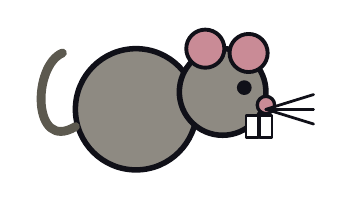
\begin{tikzpicture}[x=\Unit,y=\Unit, line join=round, line cap=round]

  % ---- background: none. A sprite sits on whatever is behind it. ----------

  % ---- body ---------------------------------------------------------------
  \fill[fur,draw=ink,line width=\Edge] (26,20) circle (\BodyR);
  % The tail, drawn before the head so the head laps over its root.
  \draw[furdark,line width=3.2pt] (12,16) .. controls (2,10) and (2,30) .. (9,33);

  % ---- head ---------------------------------------------------------------
  \fill[fur,draw=ink,line width=\Edge] (46,24) circle (10);
  \fill[pink,draw=ink,line width=1.4pt] (42,34) circle (4.4);  % ear
  \fill[pink,draw=ink,line width=1.4pt] (52,33) circle (4.4);  % ear
  \fill[ink] (51,25) circle (1.7);                             % eye
  \fill[pink,draw=ink,line width=1.2pt] (56,21) circle (2.0);  % nose

  % Two teeth, which is the whole of what the weakest rung has. Under the
  % snout and wide enough to be teeth rather than a pair of ticks.
  \foreach \x in {51.4,54.6} {
    \fill[white,draw=ink,line width=1.0pt] (\x,13.5) rectangle ++(2.8,5.0);
  }

  % ---- whiskers -----------------------------------------------------------
  \foreach \i in {1,...,\Whiskers} {
    \pgfmathsetmacro\dy{(\i-2)*3.4}
    \draw[ink,line width=1.0pt] (56,20) -- ++(\WhiskerLen,\dy);
  }

  % ---- annotations: none. --------------------------------------------------

\end{tikzpicture}
\end{document}

% ---- self-check ------------------------------------------------------------
% 1. Standalone class, compiles alone with pdflatex.
% 2. Every tunable is a \newcommand or \definecolor at the top.
% 3. \foreach draws both the teeth and the whiskers.
% 4. Order runs background -> body -> head -> whiskers -> annotations.
% 5. Circles, rectangles and one Bezier only; no external images.
